\section{Studies of signal and background separation in detector-level of cluster}
In the Future detector ,when energy of collision is upper, pileup is bigger, and the most important thing is separating signal and background efficiently. In this section, we want to study in different variables and see wether those can efficiently separate the signal and background in different detector size in detector-level of cluster.\\

Figure 3 to 5 show three variables about $c2b1$ , $\tau_{21}$, and $\tau_{32}$ in different energy of collision, the ROC curve of the different HCAL detector sizes. The criteria of separation efficiency is that in the different sizes of the detector, if the certain one of the detector size has the highest value of (1-background efficiency) at same signal efficiency of different detector sizes, it means its background efficiency is lowest, and we can say it has the highest separation efficiency compare with other detector sizes.

We can see  $c2b1$ is the best way to separation, but the detector size can't improve the separation efficiency very well.$\tau_{21}$ can't improve the separation in different detector size at 10,20,40TeV, and $\tau_{32}$ has the good pattern to follow that the smaller detector size, the better the separation efficiency.In summary, $c2b1$ and $\tau_{32}$ are two variables that can suit for the higher energy for the future analysis.\\
\label{sec:efficiency}


\begin{figure}
\begin{center}
   \subfigure[5 TeV] {
   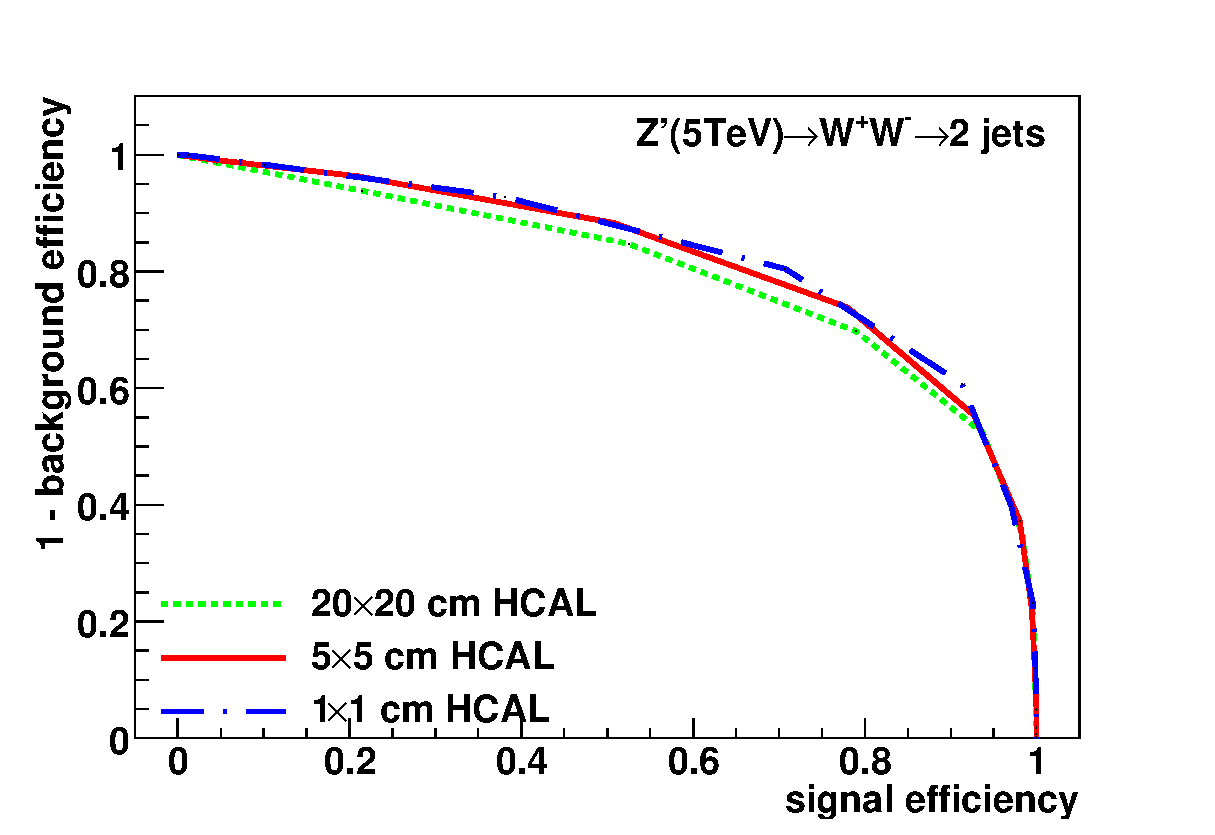
\includegraphics[width=0.43\textwidth]{figs/cluster_c2b1_5_tev_eff.eps}\hfill
   }
   \subfigure[10 TeV] {
   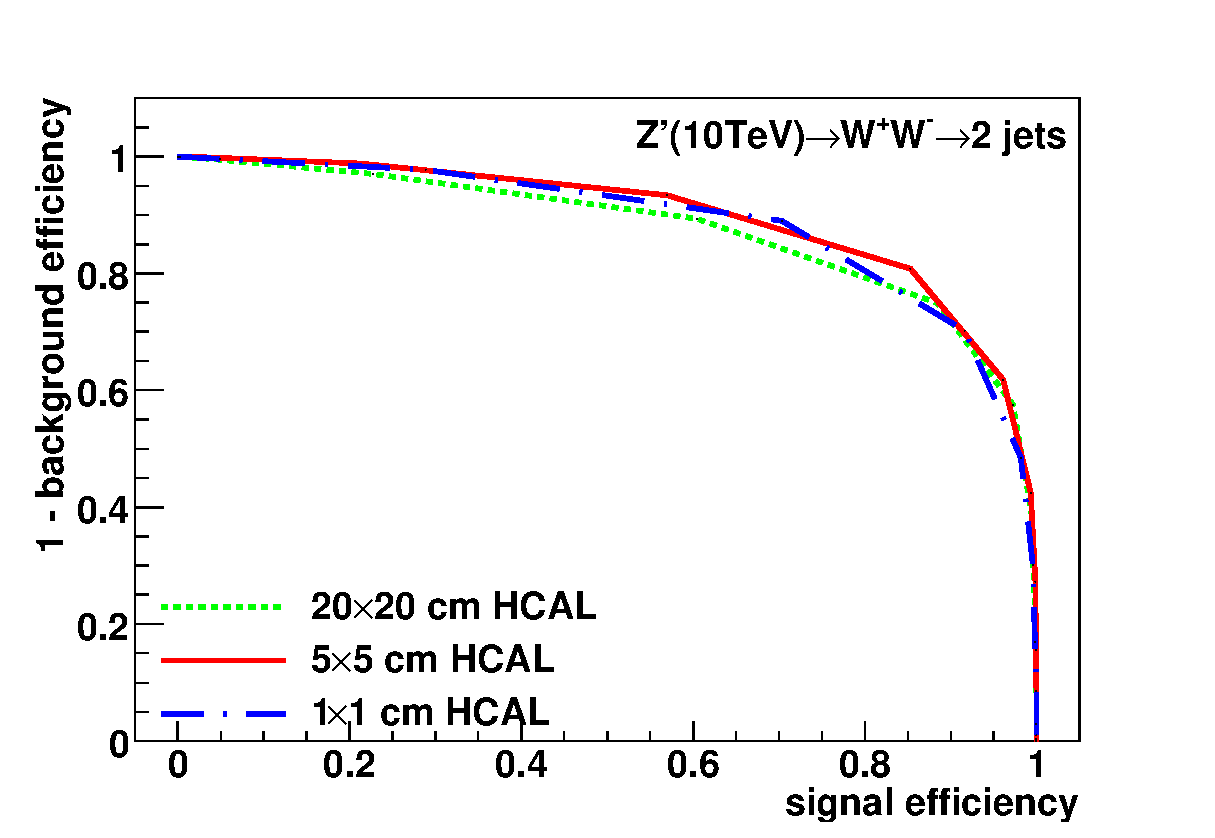
\includegraphics[width=0.43\textwidth]{figs/cluster_c2b1_10_tev_eff.eps}
   }
   \subfigure[20 TeV] {
   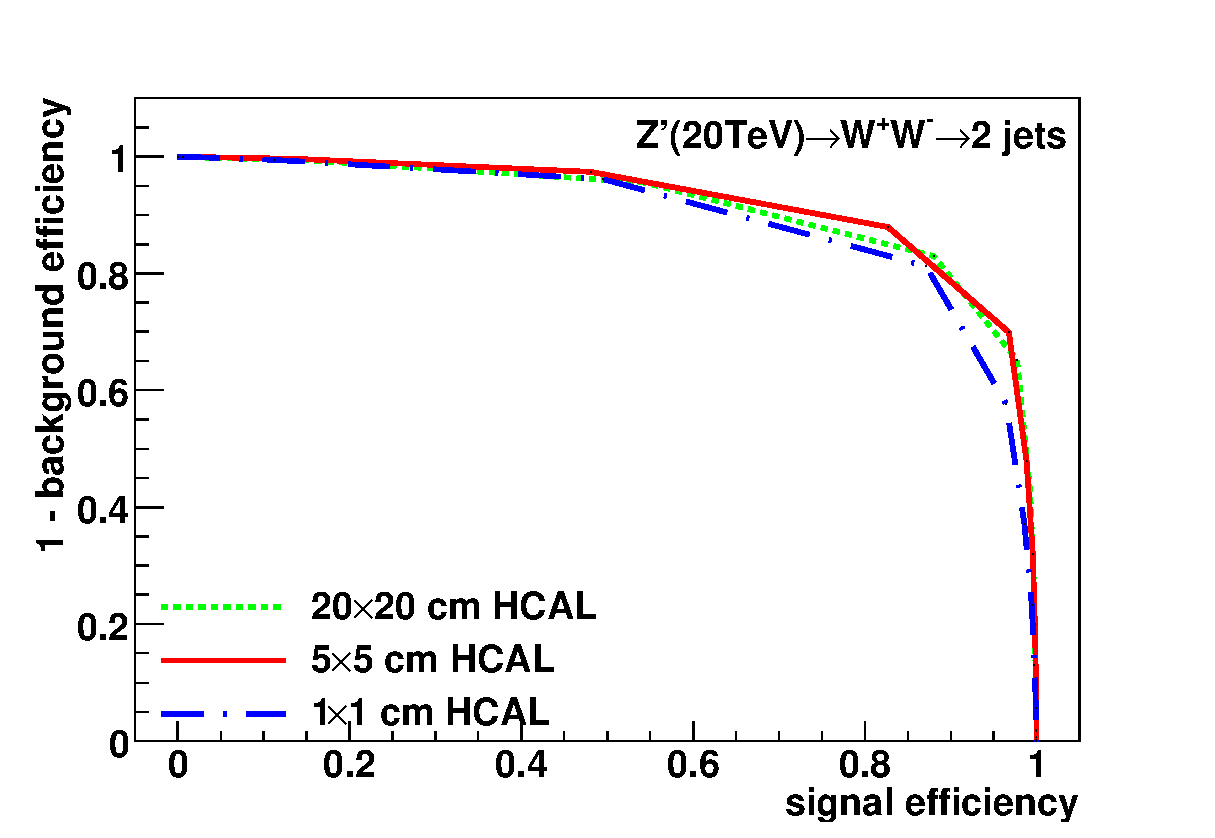
\includegraphics[width=0.43\textwidth]{figs/cluster_c2b1_20_tev_eff.eps}
   }
   \subfigure[40 TeV] {
   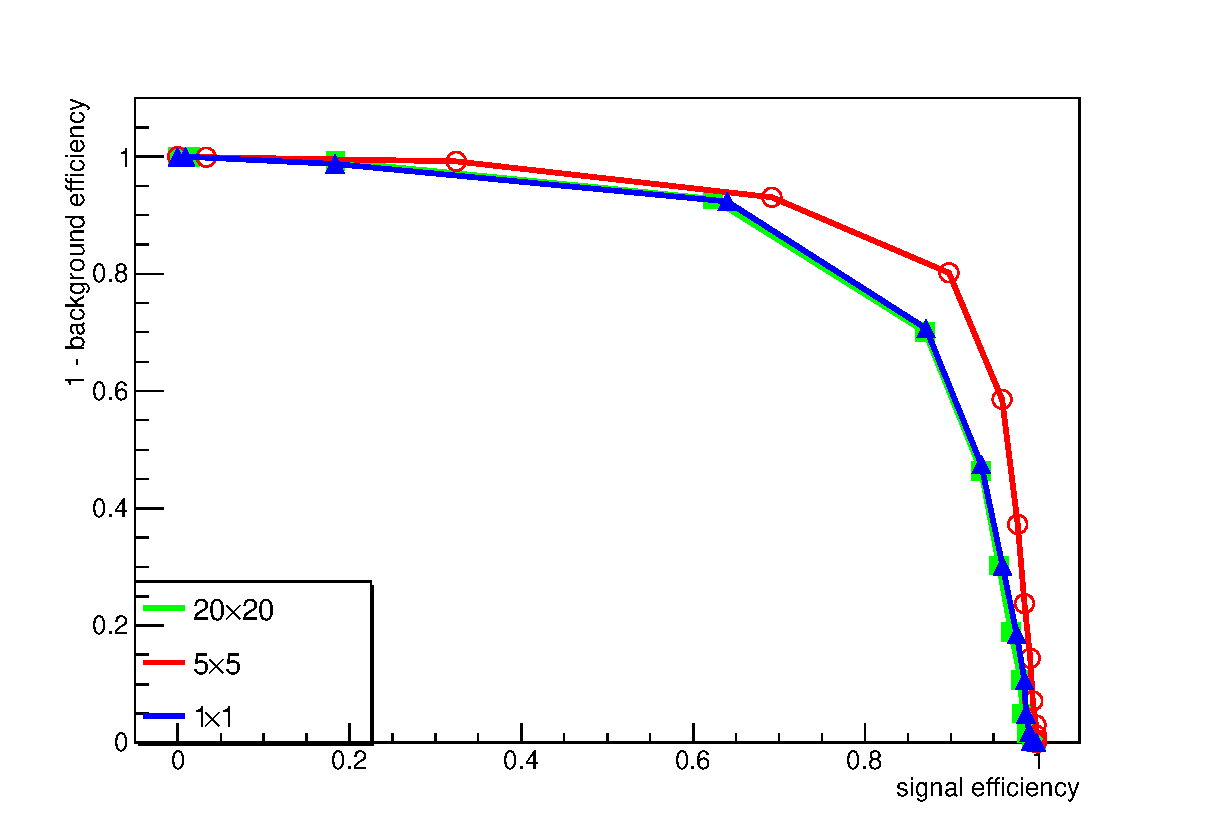
\includegraphics[width=0.43\textwidth]{figs/cluster_c2b1_40_tev_eff.eps}
   }
\end{center}
\caption{Signal efficiency versus background rejection rate using $c2b1$:This variable is the best variable to separate the signal and background, because all lines are higher than other two variables (Figure 4 and Figure 5). But in the different detector size of separation efficiency in this variable, we can't see more improvement in, as you can see, all lines nearly merge together in all energy, it means all detector sizes has the similar separation efficiency.}
\label{fig:cluster_c2b1}
\end{figure}


\begin{figure}
\begin{center}
   \subfigure[5 TeV] {
   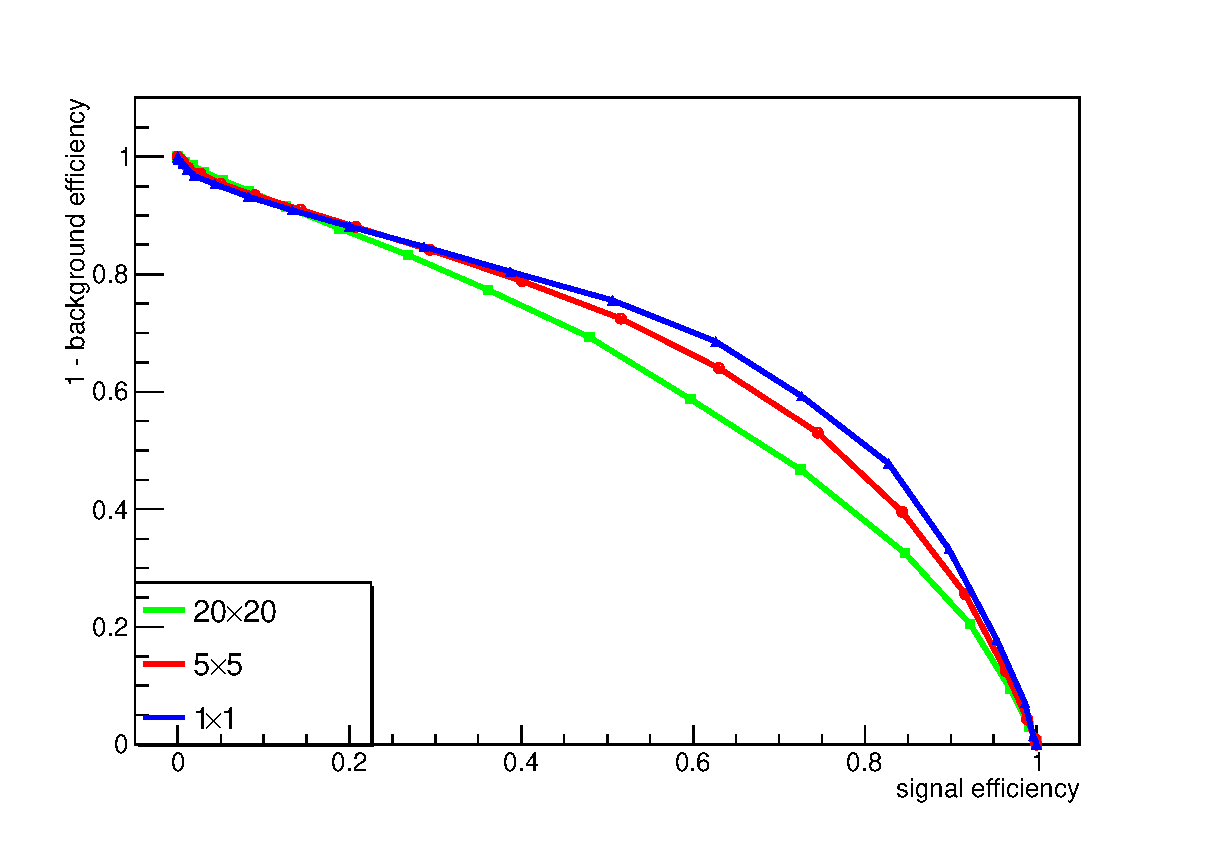
\includegraphics[width=0.43\textwidth]{figs/cluster_tau21_5_tev_eff.eps}\hfill
   }
   \subfigure[10 TeV] {
   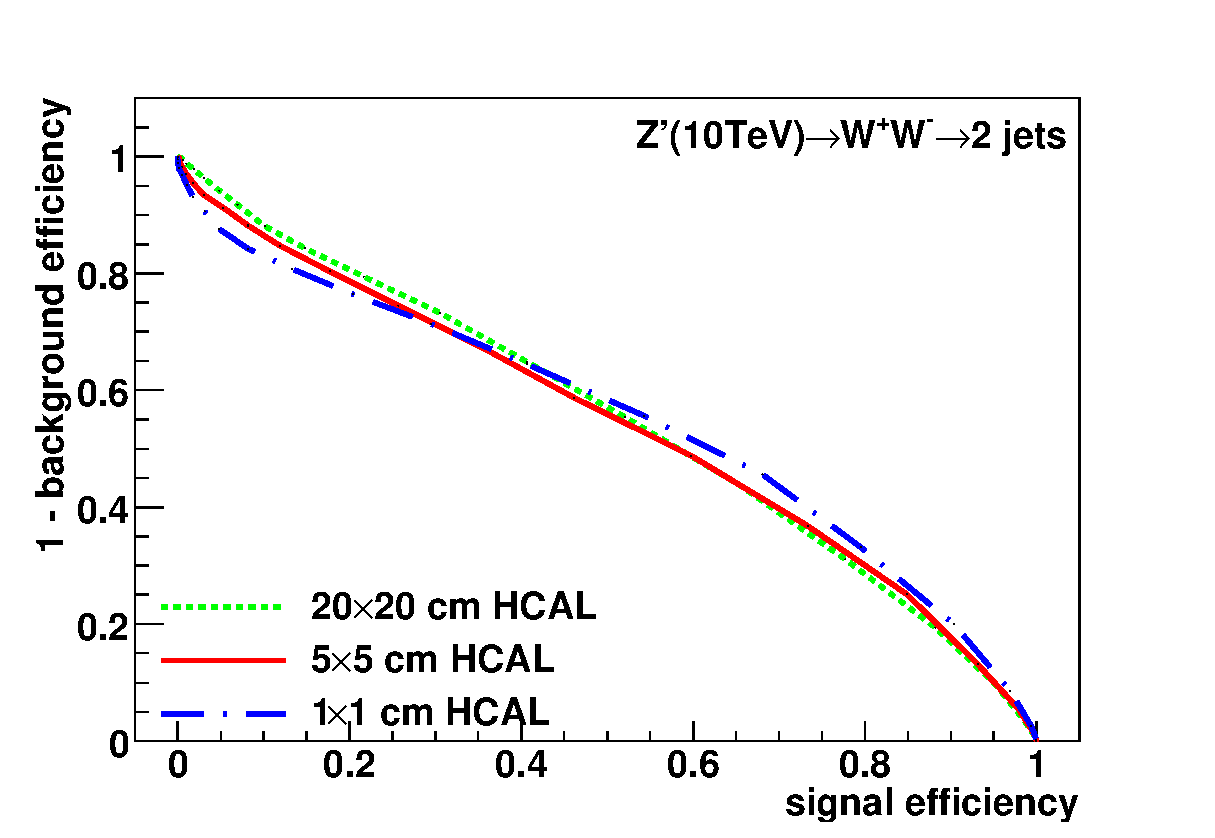
\includegraphics[width=0.43\textwidth]{figs/cluster_tau21_10_tev_eff.eps}
   }
   \subfigure[20 TeV] {
   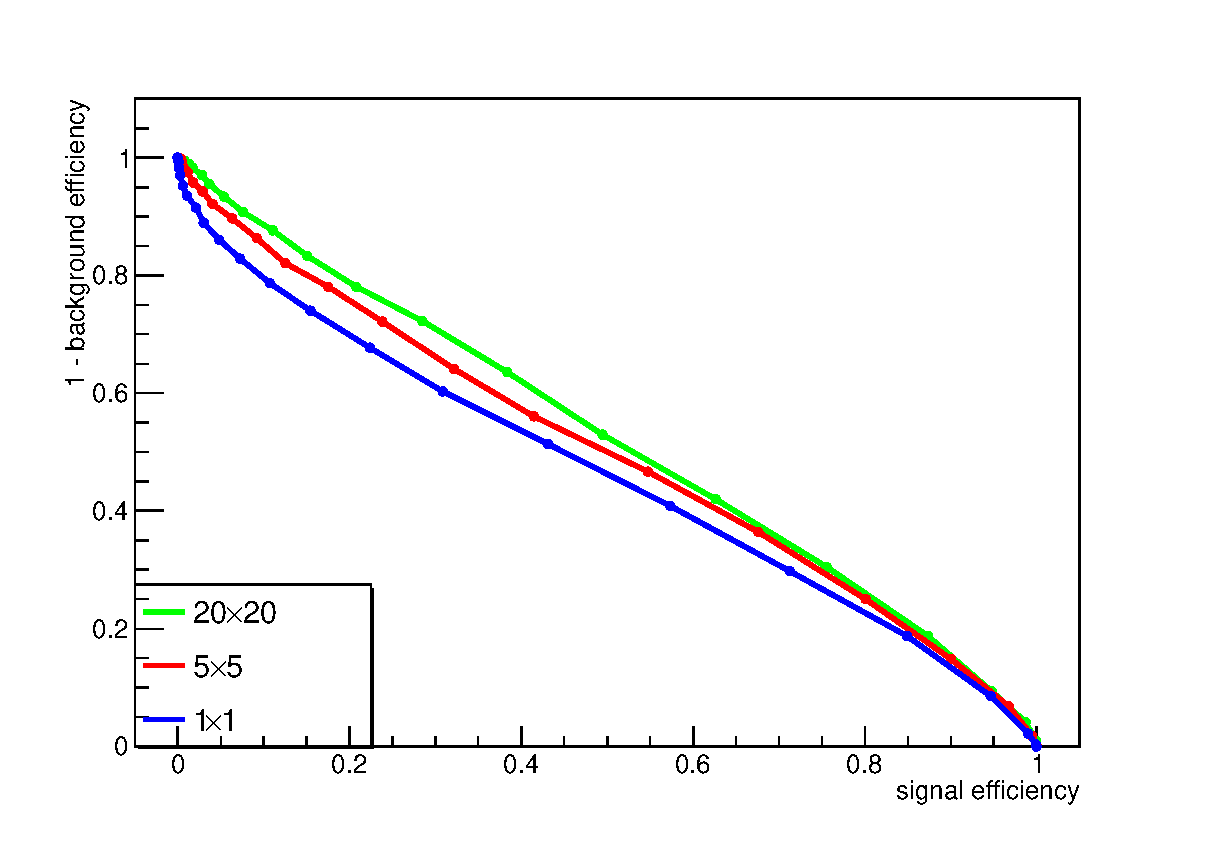
\includegraphics[width=0.43\textwidth]{figs/cluster_tau21_20_tev_eff.eps}
   }
   \subfigure[40 TeV] {
   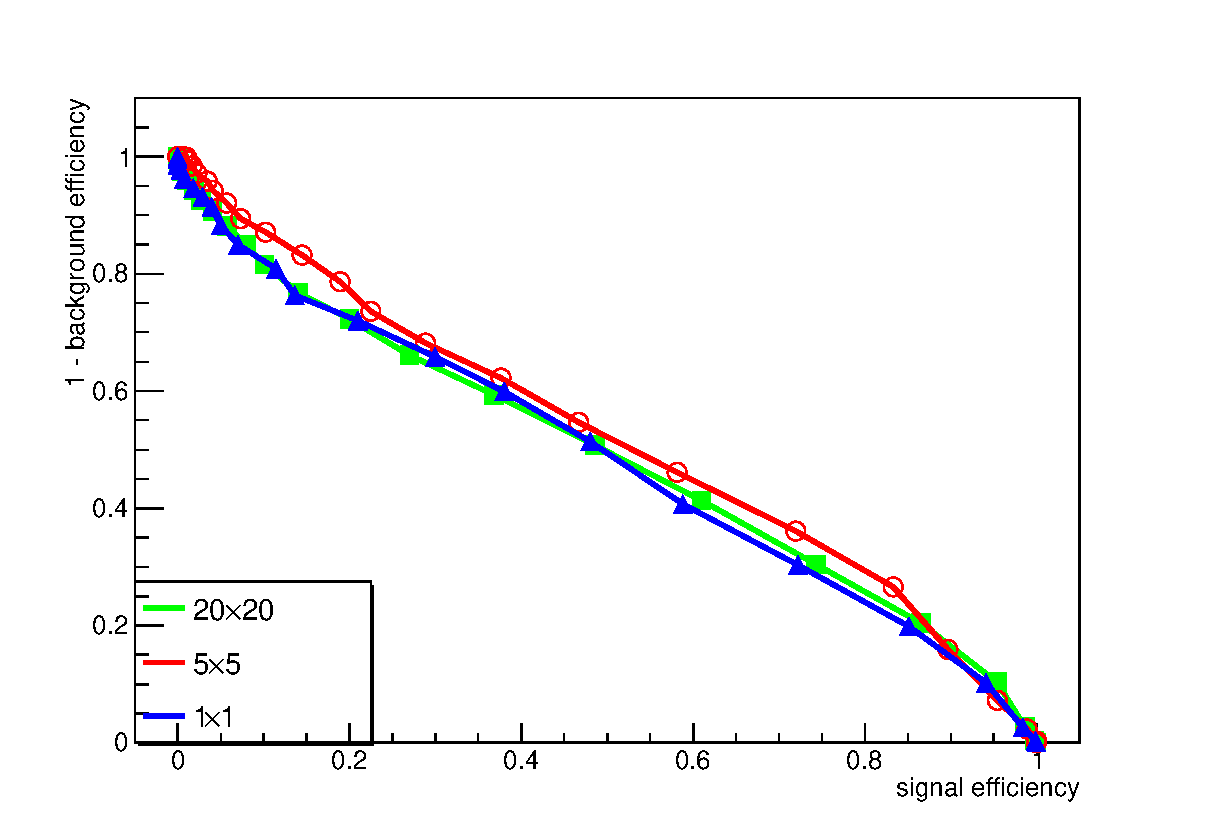
\includegraphics[width=0.43\textwidth]{figs/cluster_tau21_40_tev_eff.eps}
   }
\end{center}
\caption{Signal efficiency versus background rejection rate using $\tau_{21}$:At 5 TeV in smallest detector size(1$\times$1), it can separate signal and background well. But at 10TeV, all lines nearly merge together, they have similar separation efficiency. In 20TeV and 40TeV, we can see that it doesn't improve the separation efficiency. Specially, bigger detector size has the higher separation efficiency than smaller detector size in this two energy.}
\label{fig:cluster_tau21}
\end{figure}


\begin{figure}
\begin{center}
   \subfigure[5 TeV] {
   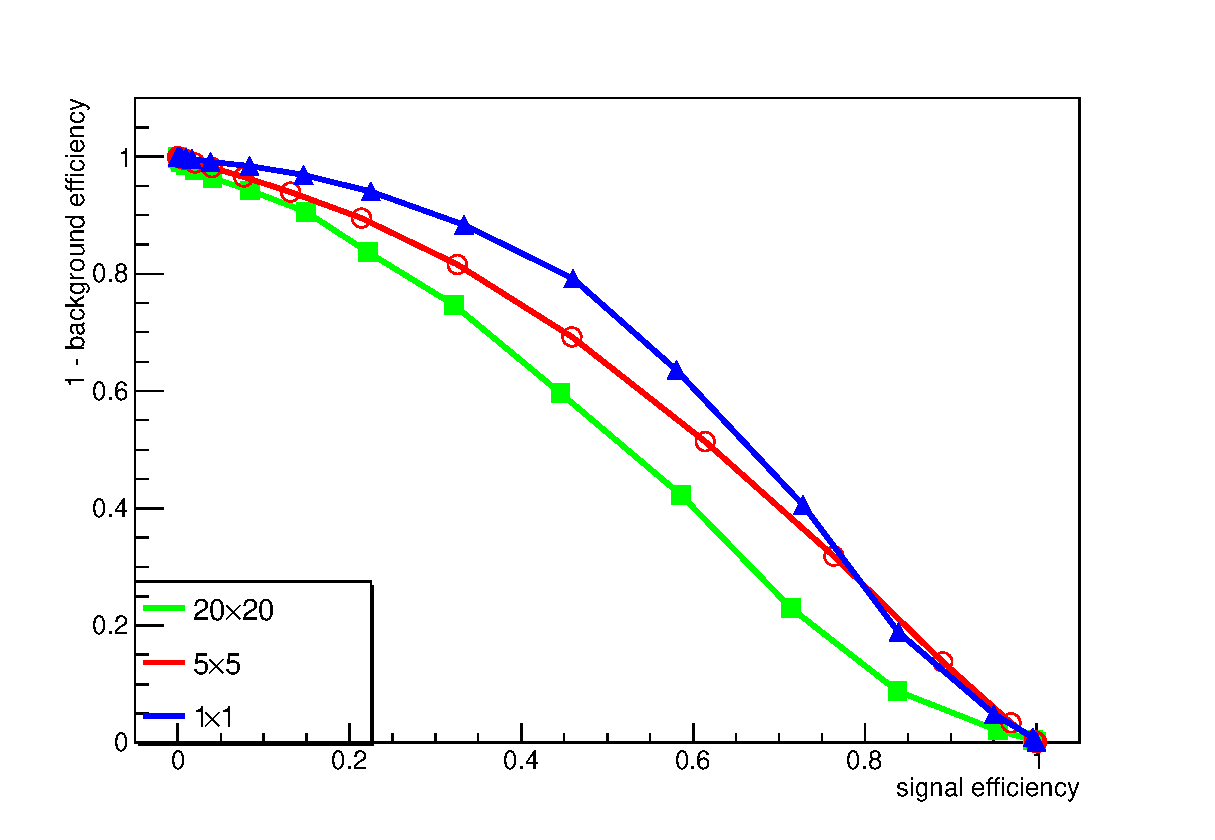
\includegraphics[width=0.43\textwidth]{figs/cluster_tau32_5_tev_eff.eps}\hfill
   }
   \subfigure[10 TeV] {
   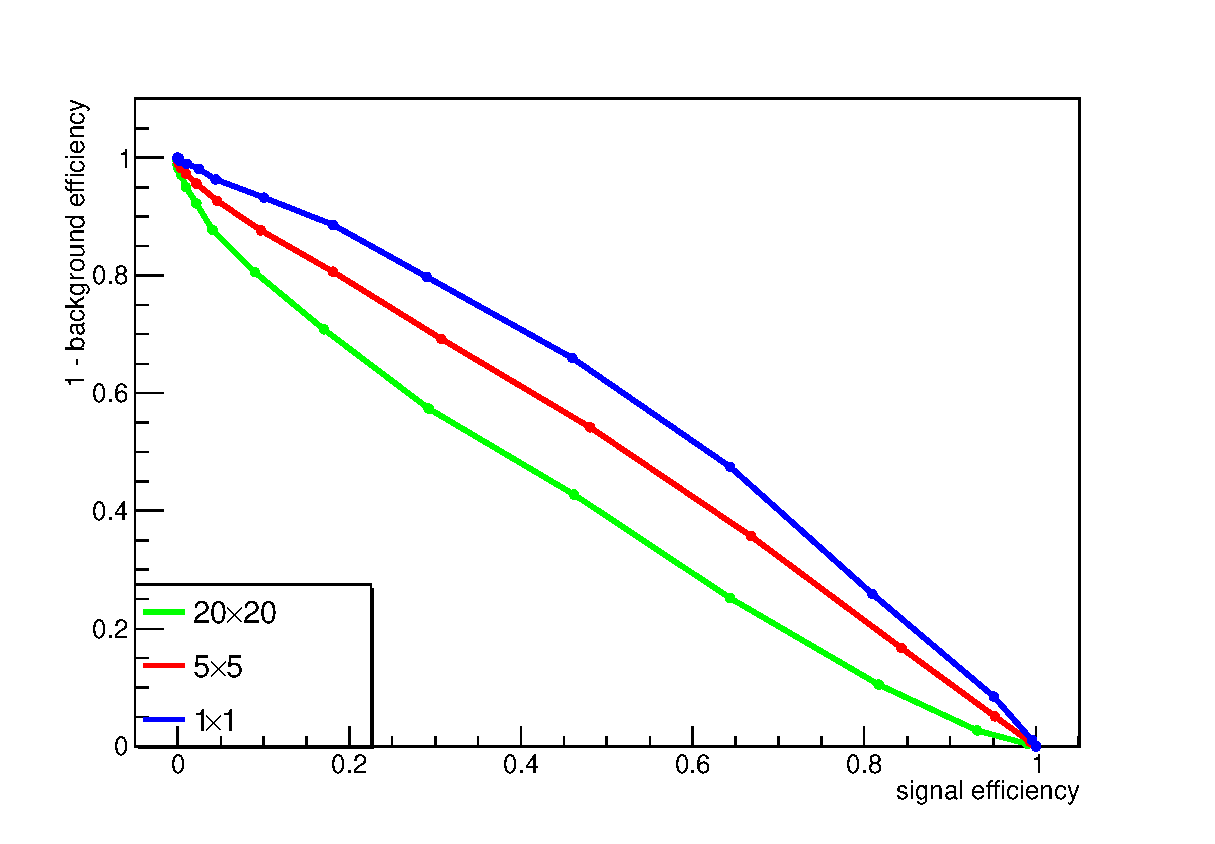
\includegraphics[width=0.43\textwidth]{figs/cluster_tau32_10_tev_eff.eps}
   }
   \subfigure[20 TeV] {
   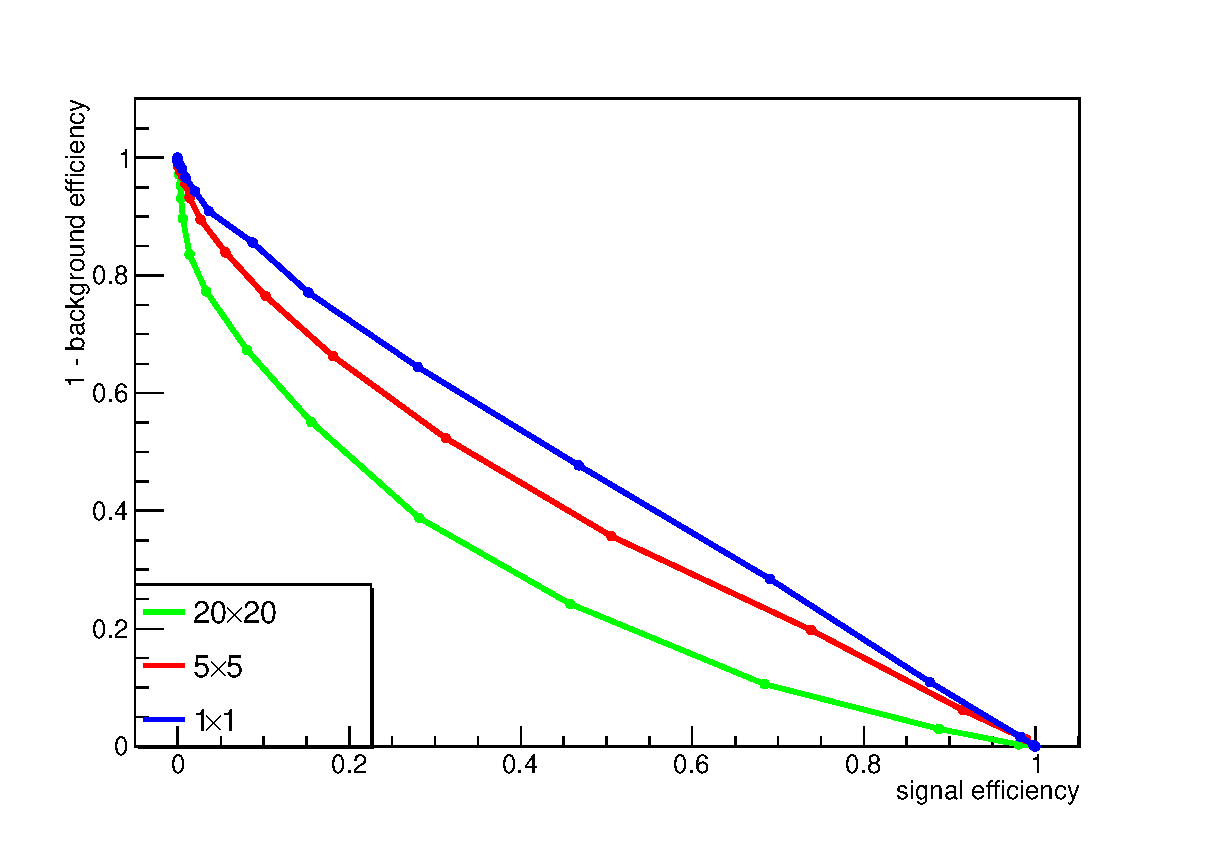
\includegraphics[width=0.43\textwidth]{figs/cluster_tau32_20_tev_eff.eps}
   }
   \subfigure[40 TeV] {
   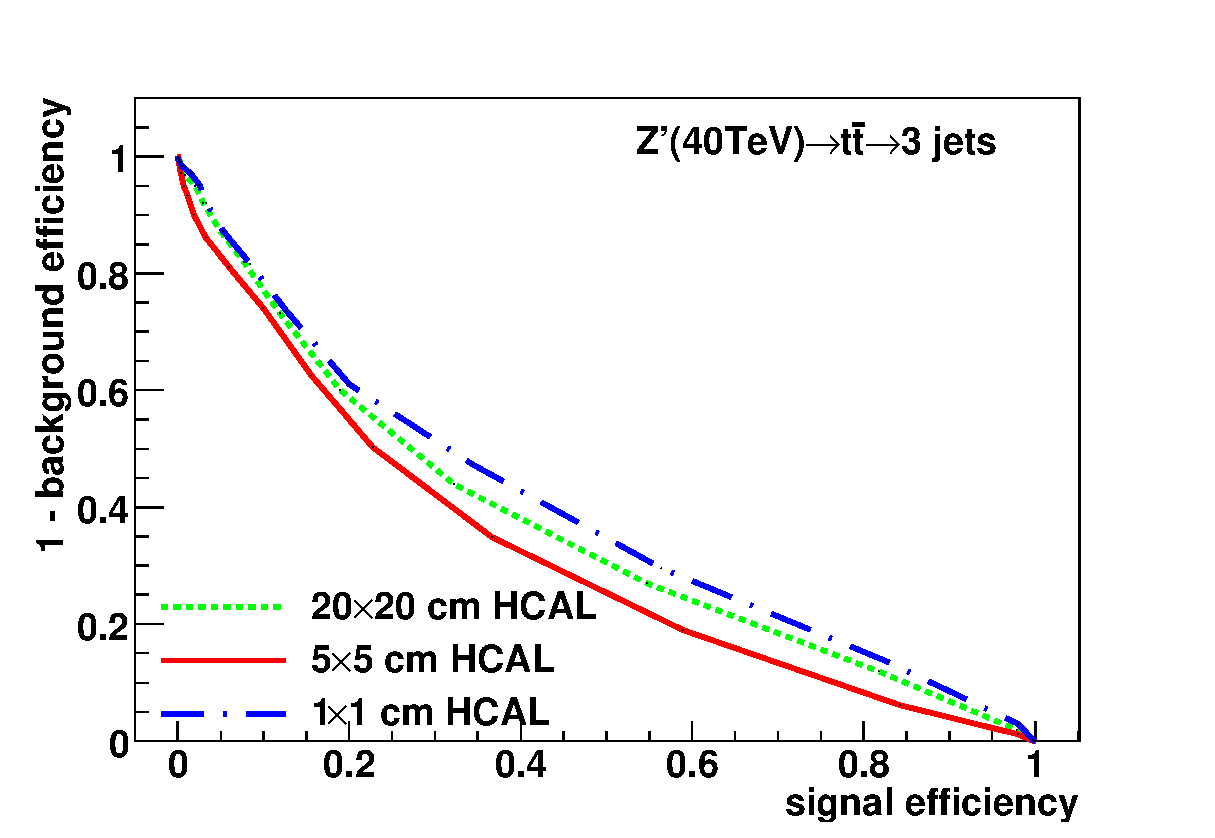
\includegraphics[width=0.43\textwidth]{figs/cluster_tau32_40_tev_eff.eps}
   }
\end{center}
\caption{Signal efficiency versus background rejection rate using $\tau_{32}$:In this variable, it's clear that it follows the role which smaller detector size have the bigger separation efficiency in all energy.}
\label{fig:cluster_tau32}
\end{figure}

